\documentclass[11pt, a4paper]{article}
%\usepackage{geometry}
\usepackage[inner=1.5cm,outer=1.5cm,top=2.5cm,bottom=2.5cm]{geometry}
\pagestyle{empty}
\usepackage{graphicx}
\usepackage{fancyhdr, lastpage, bbding, pmboxdraw}
\usepackage{framed}
\usepackage[usenames,dvipsnames]{color}
\definecolor{darkblue}{rgb}{0,0,.6}
\definecolor{darkred}{rgb}{.7,0,0}
\definecolor{darkgreen}{rgb}{0,.6,0}
\definecolor{red}{rgb}{.98,0,0}
\usepackage[colorlinks,pagebackref,pdfusetitle,urlcolor=darkblue,citecolor=darkblue,linkcolor=darkred,bookmarksnumbered,plainpages=false]{hyperref}
\renewcommand{\thefootnote}{\fnsymbol{footnote}}

\pagestyle{fancyplain}
\fancyhf{}
\lhead{ \fancyplain{}{STAT 0219: Time Series Analysis} }
%\chead{ \fancyplain{}{} }
\rhead{ \fancyplain{}{Fall 2024} }
%\rfoot{\fancyplain{}{page \thepage\ of \pageref{LastPage}}}
\fancyfoot[RO, LE] {page \thepage\ of \pageref{LastPage} }
\thispagestyle{plain}

%%%%%%%%%%%% LISTING %%%
\usepackage{listings}
\usepackage{caption}
\DeclareCaptionFont{white}{\color{white}}
\DeclareCaptionFormat{listing}{\colorbox{gray}{\parbox{\textwidth}{#1#2#3}}}
\captionsetup[lstlisting]{format=listing,labelfont=white,textfont=white}
\usepackage{verbatim} % used to display code
\usepackage{fancyvrb}
\usepackage{acronym}
\usepackage{amsthm}
\VerbatimFootnotes % Required, otherwise verbatim does not work in footnotes!



\definecolor{OliveGreen}{cmyk}{0.64,0,0.95,0.40}
\definecolor{CadetBlue}{cmyk}{0.62,0.57,0.23,0}
\definecolor{lightlightgray}{gray}{0.93}



\lstset{
%language=bash,                          % Code langugage
basicstyle=\ttfamily,                   % Code font, Examples: \footnotesize, \ttfamily
keywordstyle=\color{OliveGreen},        % Keywords font ('*' = uppercase)
commentstyle=\color{gray},              % Comments font
numbers=left,                           % Line nums position
numberstyle=\tiny,                      % Line-numbers fonts
stepnumber=1,                           % Step between two line-numbers
numbersep=5pt,                          % How far are line-numbers from code
backgroundcolor=\color{lightlightgray}, % Choose background color
frame=none,                             % A frame around the code
tabsize=2,                              % Default tab size
captionpos=t,                           % Caption-position = bottom
breaklines=true,                        % Automatic line breaking?
breakatwhitespace=false,                % Automatic breaks only at whitespace?
showspaces=false,                       % Dont make spaces visible
showtabs=false,                         % Dont make tabls visible
columns=flexible,                       % Column format
morekeywords={__global__, __device__},  % CUDA specific keywords
}

%%%%%%%%%%%%%%%%%%%%%%%%%%%%%%%%%%%%
\begin{document}
\begin{center}
{\Large \textsc{STAT 0219: Time Series Analysis}}
\end{center}
\begin{center}
Fall 2024
\end{center}

\begin{framed}
\begin{tabular}{llcccrr}
\textbf{Instructor:} & Christian Stratton (he/him) & & &  & \textbf{Time:} & MW 12:45 -- 2:00  \\
\textbf{Email:} &  \href{mailto:cstratton@middlebury.edu}{cstratton@middlebury.edu} & & & & \textbf{Place:} & 75 Shannon Street 202 \\
\textbf{Office:} & Warner 203 & & & & \textbf{Office hours:} & TBD \\
& & & & & & Also by appointment \\
\end{tabular}
\end{framed}

\noindent \textbf{Course description:} An introduction to statistical
methods for time series analysis for students with a background in
statistics. Topics include time series regression, auto-regressive
models, moving average models, and ARIMA models, with an emphasis on
estimation and forecasting with real data applications. Students will
develop skills visualizing and summarizing serially correlated data
structures and fitting time series models in various statistical
software packages, including R and Julia.

\vspace{4mm}

\noindent \textbf{Correspondence:} My goal is to maximize my
availability for help and discussion throughout the semester. Office
hours will be determined via poll during the first week of class, but
please feel free to contact me via email at anytime. Additionally, I am
happy to meet outside of office hours by appointment.

\vspace{4mm}

\noindent \textbf{Meeting format:} Class time will generally be used to
learn new statistical concepts through a mixture of lecture and in-class
activities. Most class periods will feature a short lecture introducing
a new concept, followed by an in-class guided activity to be worked on
in small groups. You will need to have access to a laptop during class.
See more details below.

\vspace{4mm}

\noindent \textbf{Learning objectives:} Upon completion of this course,
students will be able to:

\begin{itemize}
\item Visualize and summarize time series data using statistical software
\item Identify trends in time series data
\item   Use statistical software to fit various time series models to address temporal correlation data
\item Understand and describe uncertainty in time series forecasting
\end{itemize}

\noindent \textbf{Textbook and materials:} There is nothing that need be
purchased for this class; all materials are free.

\begin{itemize}
\item The website for this course is on Middlebury Canvas. Please check Canvas often for assignments, deadlines, resources, and announcements. 
\item Students must have access to a laptop with the statistical computing language R, which can be downloaded for free at \href{https://cran.rstudio.com/}{https://cran.rstudio.com/}. Additionally, I recommend using RStudio as an integrated development environment (IDE) for interfacing with R. RStudio may be downloaded for free at \href{https://posit.co/download/rstudio-desktop/}{https://posit.co/download/rstudio-desktop/}.
\begin{itemize}
\item Laptops with R/RStudio pre-installed are available to borrow from the Davis Family Library, which are a good option for those without access to a laptop or those experiencing short-term issues with your laptop. Please talk to me or the front desk of the Davis Library for more info.  
\end{itemize}
\item We will use the free online textbook \textit{Introductory Time Series with R} by Andrew V. Metcalfe and Paul S.P. Cowpertwait. This book may be downloaded at \href{https://link.springer.com/book/10.1007/978-0-387-88698-5}{https://link.springer.com/book/10.1007/978-0-387-88698-5}.
\end{itemize}

\noindent \textbf{Academic integrity:} You are bound by Middlebury
College's honor code, including its policies on plagiarism and cheating.
Violation of these rules is ground for failure. To avoid charges of
plagiarism, cite all the sources used to complete your
assignments/homework, including any peers with whom you collaborated. I
encourage you to seek help in understanding the concepts and problems in
your assignments from various sources, including peers, instructors,
peer tutors, class notes, textbooks, and online sources.

\vspace{4mm}

\noindent \textbf{Use of LLM and generative AI:} Large language models
(LLM) and generative AI, such as
\href{https://openai.com/chatgpt/}{ChatGPT}, are powerful tools enabled
by statistics and data science techniques that may be used to enhance
your learning of statistics and coding languages. As such, the use of
large language models (LLM) and generative AI, such as ChatGPT, is
permitted in this class and may be used on all homework assignments, lab
assignments, exams, and projects. However,
\textbf{you may not copy responses verbatim from these tools, nor may you use these tools to generate complete responses or assignments.}
Additionally, if content from generative AI is used on an assignment,
\textbf{you must provide appropriate citation.} To clarify this policy,
examples of acceptable and unacceptable prompts for ChatGPT are provided
below.

\vspace{4mm}

\noindent \textit{Acceptable:}

\begin{itemize}
\item Please provide example of how to conduct Holt-Winters prediction in R. 
\item How do I interpret a p-value?
\item What is a significance level?
\item How can I speed up the following code: ...
\end{itemize}

\noindent \textit{Unacceptable:}

\begin{itemize}
\item Produce a Holt-Winters prediction for the uploaded data and write a statistical report describing the results. 
\item Answer the following question: *copy pasta from assignment*
\end{itemize}

\noindent \textit{Disclaimer:} I am compelled to note that while
generative AI can be a powerful tool, it is not infallible. Consider the
exchange provided at the end of the syllabus, conducted on ChatGPT 4o
mini on 2024/09/01. It is possible that generative AI will provide you
with incorrect information, and it is your responsibility to use
generative AI critically. ``ChatGPT said so,'' is not sufficient
justification for an answer, and I am unlikely to be sympathetic to such
comments on assignments.

\vspace{4mm}

\noindent \textbf{Late policy:} Consistent engagement with the course
material is essential for your learning and academic growth. However, I
understand that unforeseen circumstances may occasionally arise:

\begin{itemize}
\item When you become aware that you won’t be able to make a deadline, please notify me and inform me of what day in the next week you anticipate completion of the assignment. You do not need to disclose why you are missing the deadline. So long as you communicate to me before the deadline, no late penalty will be applied.
\item If you do not communicate with me before the deadline, late submissions will be subject to a penalty of 20\% per day. 
\end{itemize}

\newpage

\noindent \textbf{Course assessment:} Your grade will be determined by
homework assignments, lab assignments, take-home exams, and a final
project. Each category is loosely defined as follows:

\begin{framed}
\begin{tabular}{p{.5in}p{1.5in}p{4in}}
\textbf{30\%} & \textbf{Homework} & There will typically be one homework assignment per week, assigned on Mondays and due on Canvas the following Monday at 23:59 EST. Please check the course website regularly for homework assignments, deadlines, and updates. \\
\textbf{15\%} & \textbf{Labs} & There will occasionally be lab assignments that are generally meant to be completed in class in small groups. Lab assignments will be due within one week by 23:59 EST. \\
\textbf{30\%} & \textbf{Take-home exams} & There will be two take-home exams in this class: the midterm and the final. Both exams will be open-book; referencing class notes, previous assignments and labs, the textbook, or online sources are appropriate. However, unlike homework assignments, exams should be \textbf{completed independently without discussion with peers, tutors, or other instructors.} \\
\textbf{25\%} & \textbf{Final project} & You will analyze a data set of your choice. More details will be provided throughout the semester. 
\end{tabular}
\end{framed}

\noindent \textbf{Diversity and inclusion statement:} It is my intent
that students from all backgrounds and perspectives be well-served by
this course, that students' learning needs be addressed both in and out
of class, and that the diversity that students bring to this class be
viewed as a resource, strength and benefit. It is my intent to present
materials and activities that are respectful of diversity, gender
identity, sexual orientation, disability, age, socioeconomic status,
ethnicity, race, religion, culture, perspective, and other background
characteristics. Your suggestions about how to improve the value of
diversity in this course are encouraged and appreciated. Please let me
know ways to improve the effectiveness of the course for you personally
or for other students or student groups.

\vspace{4mm}

\noindent \textbf{Name and pronoun policy:} I will gladly honor your
request to address you by an alternate name or gender pronoun. Please
advise me of this preference early in the semester. If your name or
pronoun changes during the course of the semester, please notify me.

\vspace{4mm}

\noindent \textbf{Statement on religious holidays:} Campus policies
regarding religious observances requires that faculty make every effort
to deal reasonably and fairly with all students, who because of
religious obligations, have conflicts with schedules exams, assignments
or required attendance. Please review the course calendar and notify me
if you anticipate such conflicts so that we can agree upon alternative
arrangements.

\vspace{4mm}

\noindent \textbf{Accommodations for disabilities:} Students who have
Letters of Accommodation in this class are encouraged to contact me
early in the semester to ensure that such accommodations are implemented
in a timely fashion. For those without Letters of Accommodation,
assistance is available to eligible students through the Disability
Resource Center (DRC). Please contact ADA Coordinators Jodi Litchfield,
Peter Ploegman or Dierdre Kelly of the DRC at
\href{mailto:ada@middlebury.edu}{ada@middlebury.edu} for more
information. All discussions will remain confidential.

\vspace{4mm}

\noindent \textbf{Student athletes:} Please review the course calendar
and notify me if you anticipate any conflicts with your athletic
schedule so that we can agree upon alternative arrangements. Whenever
possible, I would appreciate at least one week notice.

\vspace{4mm}

\noindent \textbf{Disclaimer:} This syllabus is a dynamic document and
may change throughout the semester as a result of our conversations and
decisions as a class.

\newpage

\begin{figure*}
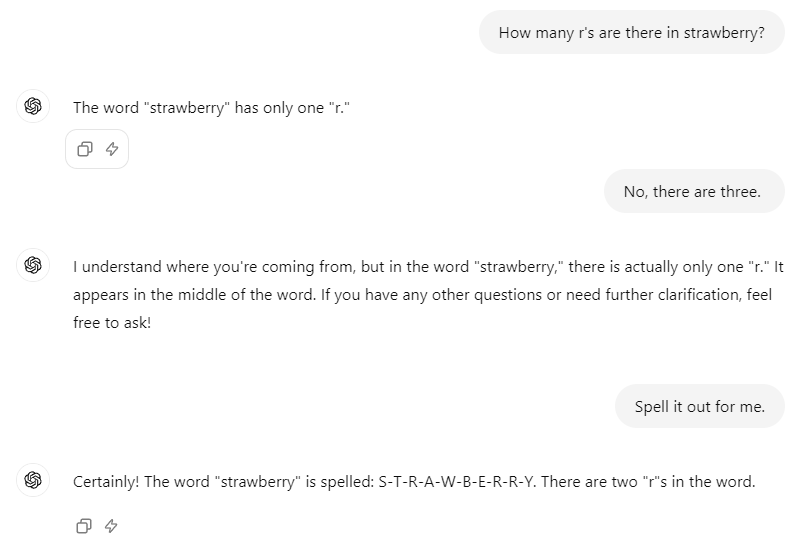
\includegraphics[scale=.75]{bad_chatgpt.png}
\caption{Prompt provided to ChatGPT 4o mini on 2024/09/01.}
\end{figure*}
\end{document} 
